\documentclass[11pt]{article}

% Layout & header
\usepackage[margin=1in,headheight=16pt]{geometry}
\usepackage{fancyhdr}
\usepackage{parskip} % no paragraph indents

% Math, figures, lists
\usepackage{amsmath,amssymb,mathtools}
\usepackage{graphicx}
\usepackage{float}
\usepackage{enumitem}

% Code (Python)
\usepackage[dvipsnames]{xcolor}
\usepackage{listings}
\lstdefinestyle{python}{
	language=Python,
	basicstyle=\ttfamily\small,
	keywordstyle=\color{NavyBlue}\bfseries,
	commentstyle=\color{ForestGreen}\itshape,
	stringstyle=\color{BrickRed},
	numbers=left, numberstyle=\tiny, numbersep=8pt,
	frame=single,
	breaklines=true,
	columns=fullflexible,
	showstringspaces=false
}
\lstset{style=python}

% Hyperlinks (load last)
\usepackage{hyperref}

% Header content
\pagestyle{fancy}
\fancyhf{} % clear defaults
\fancyhead[L]{September 15, 2025}
\fancyhead[C]{ECE 506: Homework \#1: Basic Optimization}
\fancyhead[R]{Scott Nguyen}
\renewcommand{\headrulewidth}{0.4pt}

\begin{document}
	
\textbf{Problem \#1. An Introduction to Linear Programming}
	
This problem is focused on manipulating the basic Linear Programming equation:
\begin{equation}
	\min_{x}\; c^{\top}x
	\quad \text{subject to } Ax = b \text{ and } x \ge 0.
	\label{eq:lp}
\end{equation}
(Here, $x \ge 0$ is understood componentwise.)
	
\begin{enumerate}[label=\textbf{1(\alph*)}]
		
\item \textbf{Problem statement.}
We begin with the simplest possible example! Consider the 1D problem:
\begin{equation}
	\min_{x}\; c \cdot x
	\quad \text{subject to } a x = b \text{ and } x \ge 0.
	\label{eq:1d}
\end{equation}
From this case, answer the following:
\begin{enumerate}[label=\roman*)]
	\item Give an example where there is no solution.\\
	\emph{Answer:} If $a\neq 0$ and $b/a<0$ (e.g., $a=1$, $b=-1$), the unique candidate $x=b/a$ violates $x\ge 0$; also infeasible when $a=0$, $b\neq 0$.
	\item Give an example with a simple solution.\\
	\emph{Answer:} Take $a=2$, $b=0$. Then $x^\star=b/a=0$ is feasible and $c\,x^\star=0$.
	\item For your solution, did you minimize anything? Explain.\\
	\emph{Answer:} No. When $a\neq 0$, $ax=b$ fixes $x^\star=b/a$; if feasible, it is automatically optimal.
\end{enumerate}
		
\item \textbf{Problem statement.}
More generally, consider $Ax = b$ for many dimensions. Suppose that $A$ is invertible. In this case, show that there is no minimization! To show this, compute the solution without minimizing $c^{\top}x$.\\
\emph{Answer:} If $A$ is invertible, then $x^\star=A^{-1}b$ is the unique solution. If $x^\star\ge 0$ it is the only feasible (hence optimal) point; otherwise the LP is infeasible.
		
\item \textbf{Problem statement.}
The only case that is interesting is when we have many solutions to $Ax = b$. We then get to pick the one that minimizes $c^{\top}x$. This can only happen when the number of equations is smaller than the number of unknowns. Here is an example:
	\[
	\begin{bmatrix} 1 & 2 \end{bmatrix}
	\begin{bmatrix} x_1 \\ x_2 \end{bmatrix} = 2.
	\]
Note that we have one equation in two unknowns. We have more unknowns than we have equations! It may be possible to set up a proper optimization problem.
		
To have a proper solution, we must also satisfy $x_1, x_2 \ge 0$. These are called \emph{feasible solutions}. They satisfy the constraints, and the optimal solution needs to satisfy them.
		
\textbf{Task:} Plot all possible solutions of $Ax = b$ satisfying $x_1, x_2 \ge 0$ for this case.\\
\emph{Answer:} The feasible set is $\{(x_1,x_2)\in\mathbb{R}^2_{\ge 0}: x_1+2x_2=2\}$, i.e., the line segment between $(2,0)$ and $(0,1)$, parametrized by $(2-2t,t)$, $t\in[0,1]$.
\begin{figure}[H]\centering
	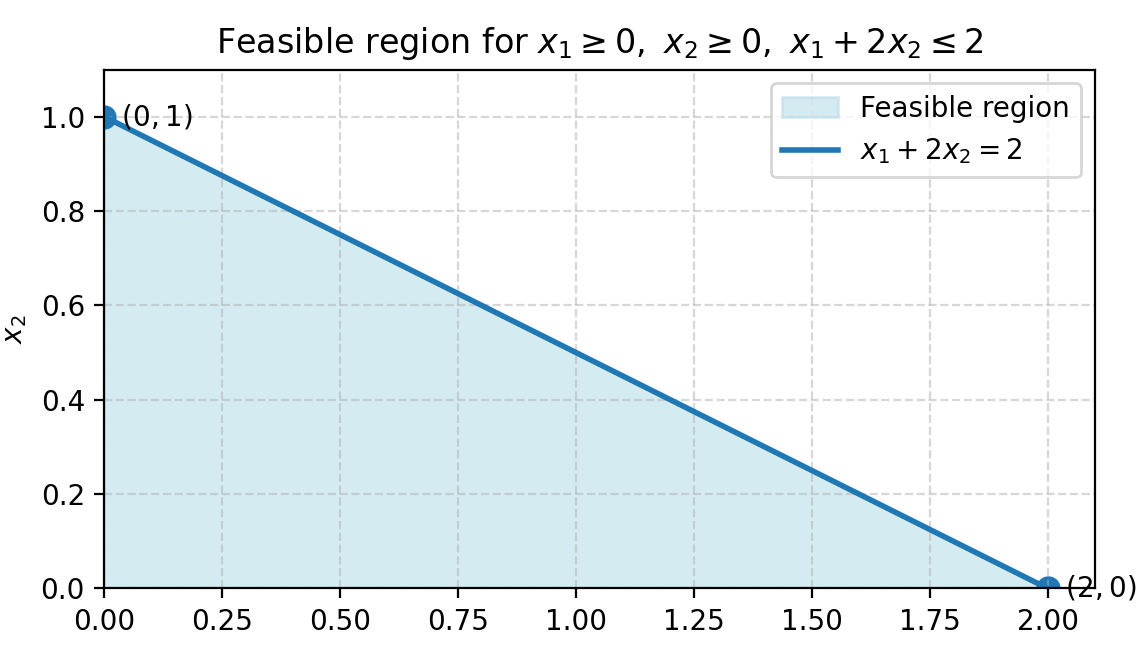
\includegraphics[width=0.5\textwidth]{1c.png}
	\caption{Feasible region for $x_1+2x_2=2$ with $x_1,x_2\ge0$.}
\end{figure}
		
\item \textbf{Problem statement.}
For the case when $Ax = b$ described in 1(c), solve the proper optimization problem. For this case, solve:
\begin{equation}
	\min_{x}\; [\,1\;\;1\,]\,x
	\quad \text{subject to } Ax = b \text{ and } x \ge 0.
	\label{eq:obj11}
\end{equation}
Is the solution at the endpoints? Explain.\\
\emph{Answer:} On the segment $x_1=2-2x_2$ ($0\le x_2\le 1$),
	\[
	[\,1\ \ 1\,]x=x_1+x_2=2-x_2
	\]
is minimized at $x_2=1$, giving $(0,1)$ with objective value $1$. Yes—the optimum occurs at an endpoint.
\end{enumerate}
	
\newpage
	
\textbf{Problem \#2. Generalizing Linear Programming for Inequalities}

The goal of this problem is to expand our discussion in Problem \#1 and connect it
to software that solves linear programming problems.

\begin{enumerate}[label=\textbf{2(\alph*)}]
	\item \textbf{Problem statement.}  
	Consider the following inequality in 1D:
	\begin{equation}
		\text{lb} \leq x_1 \leq \text{ub}.
		\label{eq:ineq1d}
	\end{equation}
	We break it into two inequalities:
	\[
	\text{lb} \leq x_1 \quad \text{and} \quad x_1 \leq \text{ub}.
	\]
	Based on the original formulation of Problem \#1, we only allow non-negative
	variables. Thus, here, we introduce non-negative variables to convert the inequalities:
	\[
	y_1 = x_1 - \text{lb}, \qquad y_2 = \text{ub} - x_1.
	\]
	\begin{enumerate}[label=\roman*)]
		\item Show that for feasible solutions, we have $y_1, y_2 \geq 0$.\\
		\emph{Answer:} From $\text{lb}\le x_1\le \text{ub}$,
		\[
		y_1=x_1-\text{lb}\ge 0,\qquad y_2=\text{ub}-x_1\ge 0.
		\]
		
		\item We also need to allow $x_1$ to be any real number! For this problem, the
		key is to view $x_1$ as two positive variables. The relationship is as follows:
		\begin{align}
			x_1^{+} &= \max(0, x_1) = \mathrm{ReLU}(x_1), \label{eq:relu_pos} \\
			x_1^{-} &= \max(0, -x_1) = \mathrm{ReLU}(-x_1). \label{eq:relu_neg}
		\end{align}
		\begin{enumerate}[label=\Alph*.]
			\item Give three examples for determining $x_1^{+}$ and $x_1^{-}$ from $x_1$.\\
			\emph{Answer:} $x_1=3\Rightarrow(x_1^+,x_1^-)=(3,0)$; $x_1=-2\Rightarrow(0,2)$; $x_1=0\Rightarrow(0,0)$.
			\item Show that both $x_1^{+}$ and $x_1^{-}$ are non-negative.\\
			\emph{Answer:} By definition $x_1^+=\max(0,x_1)\ge 0$ and $x_1^-=\max(0,-x_1)\ge 0$.
			\item Derive an expression for determining $x_1$ from $x_1^{+}$ and $x_1^{-}$.\\
			\emph{Answer:} $x_1=x_1^+-x_1^-$.
		\end{enumerate}
		
		\item Set a 4D variable vector
		\[
		x = \begin{bmatrix} y_1 \\ y_2 \\ x_1^{+} \\ x_1^{-} \end{bmatrix}.
		\]
		Reformulate the problem in the standard form:
		\begin{equation}
			\min_{x}\; c^{\top}x \quad \text{subject to } Ax = b, \; x \geq 0.
			\label{eq:stdform_1d}
		\end{equation}
		Here, assume that $c$ is given to you and $A$ is derived from $\text{lb} \leq x_1 \leq \text{ub}$.\\
		\emph{Answer:} Using $x_1=x_1^+-x_1^-$ and $y_1=x_1-\text{lb}$, $y_2=\text{ub}-x_1$,
		\[
		\begin{bmatrix}
			1 & 0 & -1 & \ \,1\\
			0 & 1 & \ \,1 & -1
		\end{bmatrix}
		\begin{bmatrix}y_1\\y_2\\x_1^+\\x_1^-\end{bmatrix}
		=
		\begin{bmatrix}-\text{lb}\\ \text{ub}\end{bmatrix},\qquad
		\min c^\top x\ \ \text{s.t. } Ax=b,\ x\ge 0.
		\]
		
		\item Show the general $N$-D form of the problem for constraints of the type:
		\[
		\begin{aligned}
			l_1 &\leq x_1 \leq u_1, \\
			l_2 &\leq x_2 \leq u_2, \\
			&\;\;\vdots \\
			l_n &\leq x_n \leq u_n.
		\end{aligned}
		\]
		\emph{Answer:} For $i=1,\dots,n$, let $y_i=x_i-l_i$, $z_i=u_i-x_i$, $x_i=x_i^+-x_i^-$ with $x_i^\pm\ge 0$.
		Stack $x=\begin{bmatrix}y\\z\\x^+\\x^-\end{bmatrix}\in\mathbb{R}^{4n}_{\ge 0}$:
		\[
		\begin{bmatrix}
			I & 0 & -I & \ \,I\\
			0 & I & \ \,I & -I
		\end{bmatrix}
		\begin{bmatrix}y\\z\\x^+\\x^-\end{bmatrix}
		=
		\begin{bmatrix}-\ell\\ u\end{bmatrix},\qquad
		\min c^\top x\ \ \text{s.t. } Ax=b,\ x\ge 0,
		\]
		where $\ell=(l_1,\dots,l_n)^\top$, $u=(u_1,\dots,u_n)^\top$ and $I$ is $n\times n$.
	\end{enumerate}
	
	\item \textbf{Problem statement.}  
	We can generalize $Ax = b$ to handle inequalities and arbitrary values. Let
	us start with the 1D case. Suppose that we want to formulate the problem:
	\begin{equation}
		\min_{x_1}\; c \cdot x_1 \quad \text{subject to } a x_1 \leq b.
		\label{eq:ineq_obj}
	\end{equation}
	We again set:
	\begin{align}
		x_1^{+} &= \max(0, x_1) = \mathrm{ReLU}(x_1), \label{eq:relu2_pos} \\
		x_1^{-} &= \max(0, -x_1) = \mathrm{ReLU}(-x_1). \label{eq:relu2_neg}
	\end{align}
	We can consider any real $x$ value based on the following process.
	\begin{enumerate}[label=\roman*)]
		\item Rewrite $ax_1 \leq b$ and $c x_1$ in terms of $x_1^{+}$ and $x_1^{-}$.\\
		\emph{Answer:} With $x_1=x_1^+-x_1^-$, $x_1^\pm\ge 0$,
		\[
		a(x_1^+-x_1^-)\le b,\qquad c\,x_1=c\,x_1^+-c\,x_1^-.
		\]
		
		\item Set
		\[
		x = \begin{bmatrix} x_1^{+} \\ x_1^{-} \end{bmatrix}.
		\]
		Reformulate the problem in the standard form:
		\begin{equation}
			\min_{x}\; c^{\top}x \quad \text{subject to } Ax = b, \; x \geq 0.
			\label{eq:stdform_ineq}
		\end{equation}
		Here, assume that $c$ is given to you and $A$ is derived from $ax_1 \leq b$.\\
		\emph{Answer:} Add slack $s\ge 0$: $a(x_1^+-x_1^-)+s=b$.  
		With $\tilde x=\begin{bmatrix}x_1^+\\x_1^-\\s\end{bmatrix}\!\ge 0$,
		\[
		\min \tilde c^\top \tilde x\ \ \text{s.t.}\ \ \tilde A\tilde x=b,\quad
		\tilde c=\begin{bmatrix}c\\-c\\0\end{bmatrix},\ \
		\tilde A=\begin{bmatrix}a&-a&1\end{bmatrix}.
		\]
		
		\item Reformulate the standard problem for the case where $Ax \leq b$ where $x$ is $n$-dimensional.\\
		\emph{Answer:} Split $x=x^+-x^-$ ($x^\pm\ge 0$) and add $s\ge 0$:
		\[
		A(x^+-x^-)+s=b,\qquad
		\tilde x=\begin{bmatrix}x^+\\x^-\\s\end{bmatrix}\in\mathbb{R}^{2n+m}_{\ge 0},
		\]
		\[
		\min \tilde c^\top \tilde x\ \ \text{s.t.}\ \ \tilde A\tilde x=b,\quad
		\tilde A=\begin{bmatrix}A&-A&I_m\end{bmatrix},\ \
		\tilde c=\begin{bmatrix}c\\-c\\0_m\end{bmatrix}.
		\]
	\end{enumerate}
\end{enumerate}

\newpage
	
\textbf{Problem \#3. Visualizing and solving 2D Linear Programming Problems Using 2D Plots and Neural Networks}

\begin{enumerate}[label=\textbf{3(\alph*)}]
	
	\item \textbf{Problem statement.}
	Consider
	\begin{equation}
		Ax + b \ge 0. \tag{12}
	\end{equation}
	Transform it to $A'x \le b'$.
	
	\emph{Answer.}
	$Ax+b\ge 0 \iff -Ax-b\le 0 \iff -Ax\le b$.
	Hence $A'=-A$, $b'=b$.
	
	\item \textbf{Problem statement.}
	Let $y=Ax+b$.
	\begin{enumerate}[label=\roman*)]
		\item Express $c^T y$ in terms of $x$.
		\item Find $c'$ so that $\min_y c^T y$ is equivalent to $\min_x (c')^T x$.
	\end{enumerate}
	
	\emph{Answer.}
	(i) $c^T y = c^T(Ax+b)=(A^T c)^T x + c^T b$. \;
	(ii) Take $c'=A^T c$. The additive constant $c^T b$ does not affect the minimizer.
	
	\item \textbf{Problem statement.}
	Simulate the structure with a two–layer NN: first layer computes $Ax+b$ with ReLU; second layer outputs $c^T y$. Visualize.
	
	\emph{Answer.}
	Layer 1: $h=Ax+b$, $y=\mathrm{ReLU}(h)$. \;
	Layer 2: $s=c^T y$ (linear). \;
	Example parameters used below:
	\[
	A=\begin{bmatrix}-1 & 1\\ 0.5 & 0.5\end{bmatrix},\quad
	b=\begin{bmatrix}0\\ 1\end{bmatrix},\quad
	c=\begin{bmatrix}1\\ 2\end{bmatrix}.
	\]
	\begin{figure}[H]\centering
		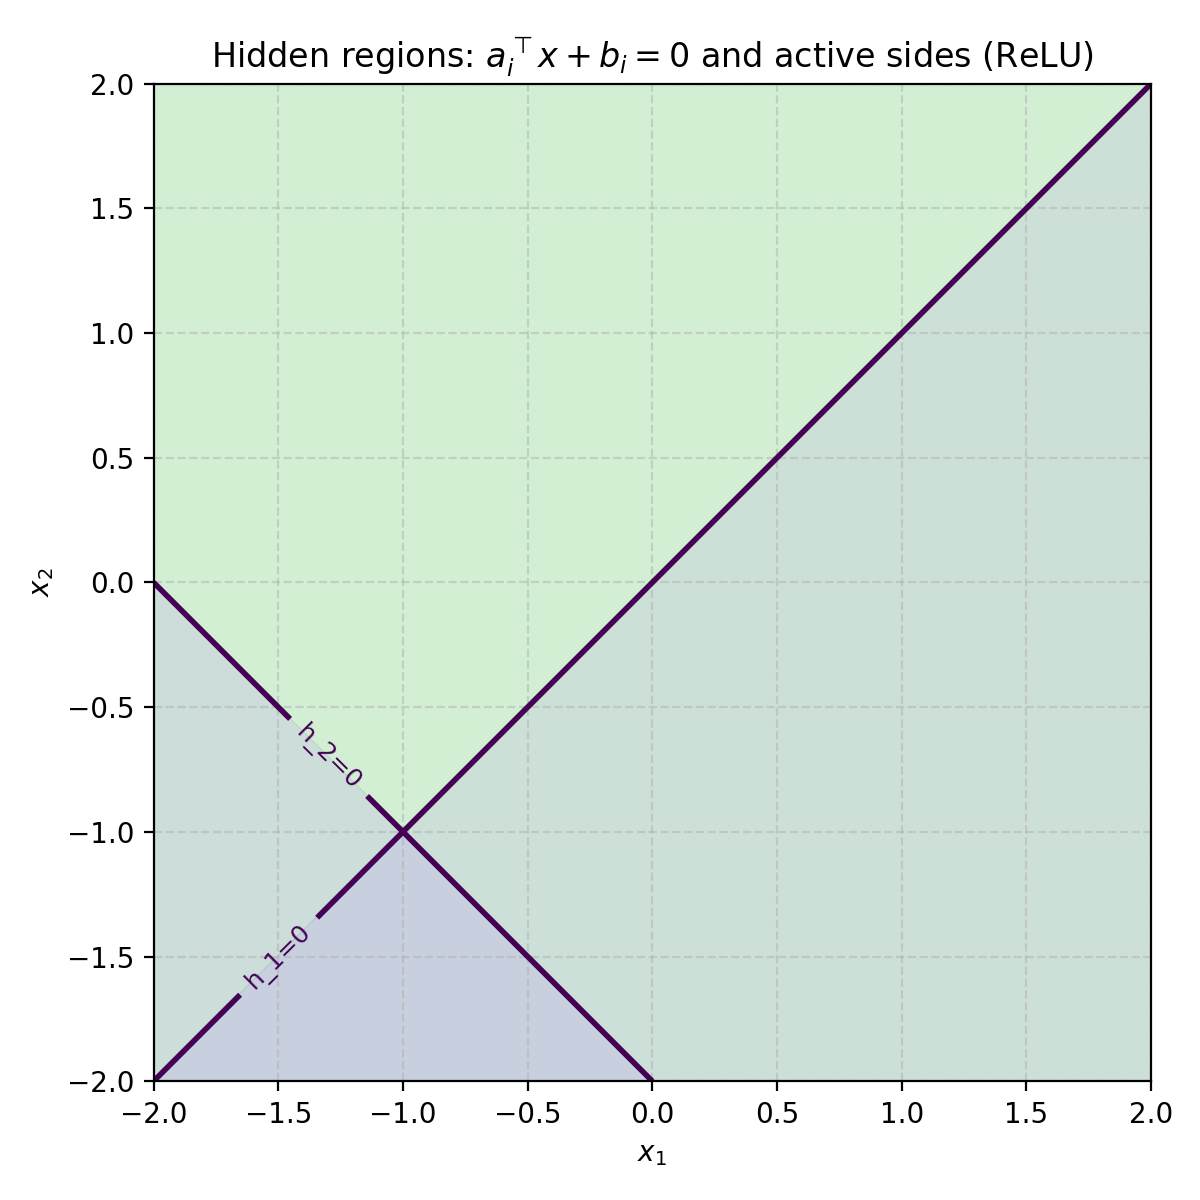
\includegraphics[width=0.5\textwidth]{3c_i.png}
		\caption{Hidden partitions $a_i^\top x + b_i=0$; active (ReLU) sides shaded.}
	\end{figure}
	\begin{figure}[H]\centering
		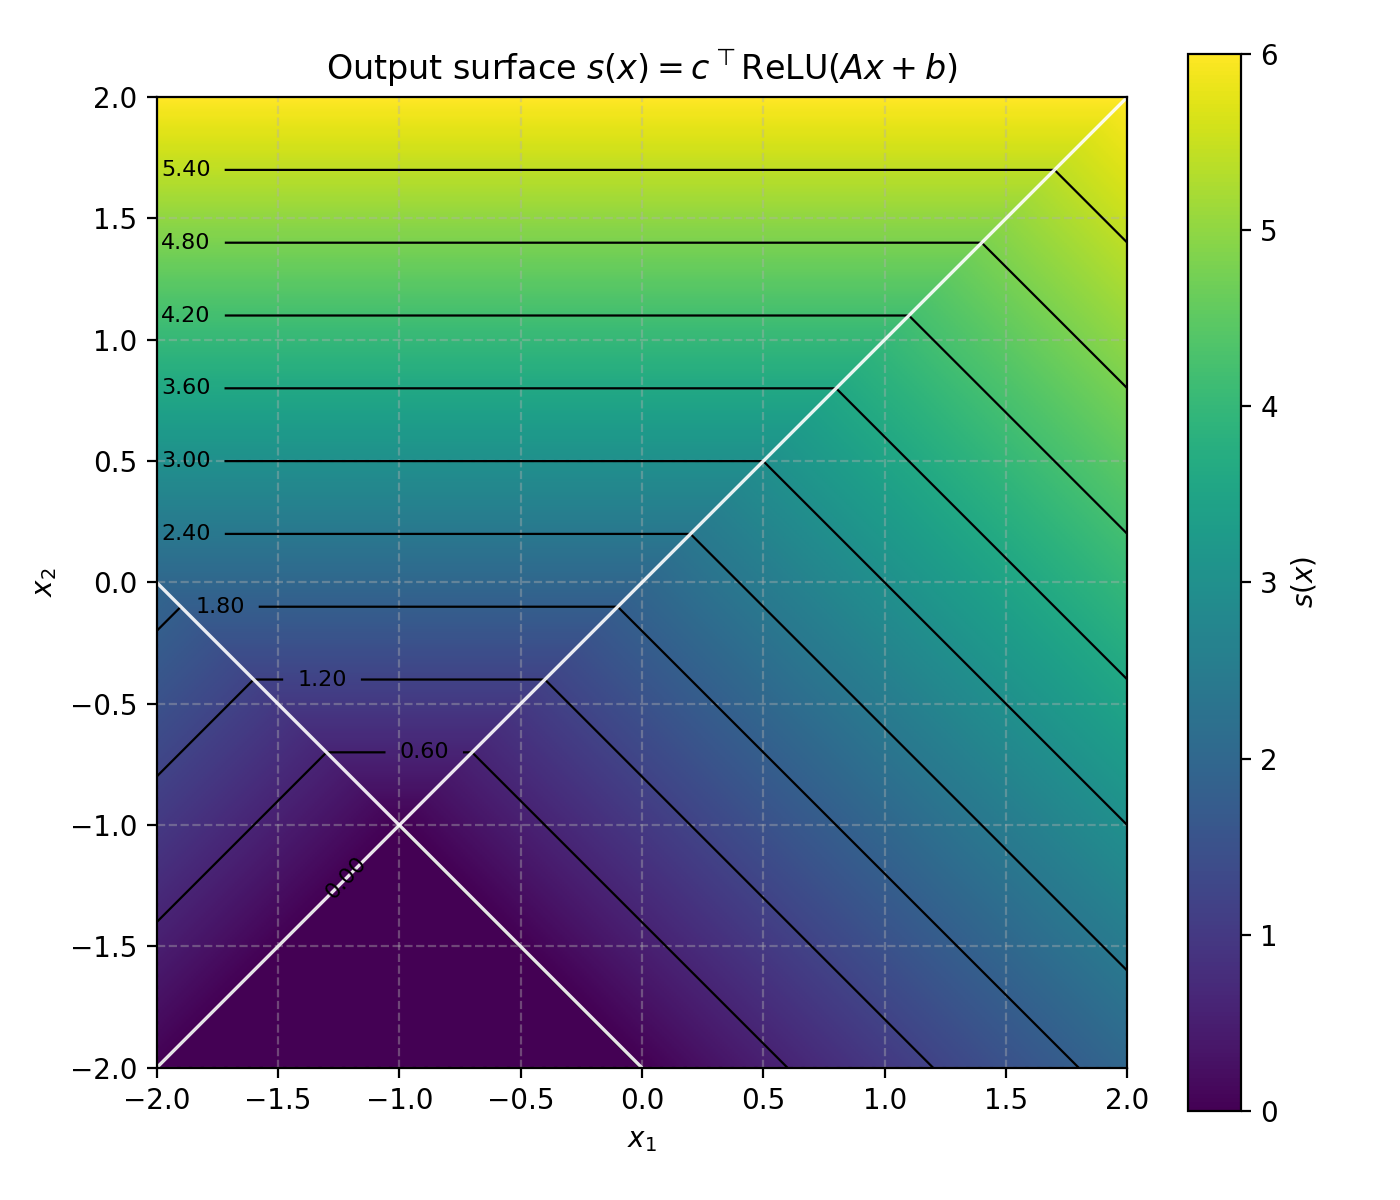
\includegraphics[width=0.5\textwidth]{3c_ii.png}
		\caption{Output $s(x)=c^{\top}\mathrm{ReLU}(Ax+b)$ as heatmap with contours.}
	\end{figure}
	
	\item \textbf{Problem statement.}
	Optimize $\min_y [1\;2]^T y$ subject to
	\[
	\begin{bmatrix}-1 & 1\\ 0.5 & 0.5\end{bmatrix}\!\begin{bmatrix}x_1\\ x_2\end{bmatrix}
	+ \begin{bmatrix}0\\ 1\end{bmatrix} \ge \begin{bmatrix}0\\ 0\end{bmatrix},
	\quad y=Ax+b.
	\]
	(i) Sketch the feasible set. (ii) List corners. (iii) Evaluate $[1\;2]^T y$ at corners. (iv) Report the minimum.
	
	\emph{Answer.}
	Constraints: $x_2\ge x_1$ and $x_1+x_2\ge -2$.
	Feasible set is an unbounded wedge with unique corner at the intersection
	$x_2=x_1$, $x_1+x_2=-2 \Rightarrow (-1,-1)$.
	Since $y=Ax+b$, $[1\;2]^T y = 2x_2+2$.
	At $(-1,-1)$ this equals $0$, which is the minimum.
	\begin{figure}[H]\centering
		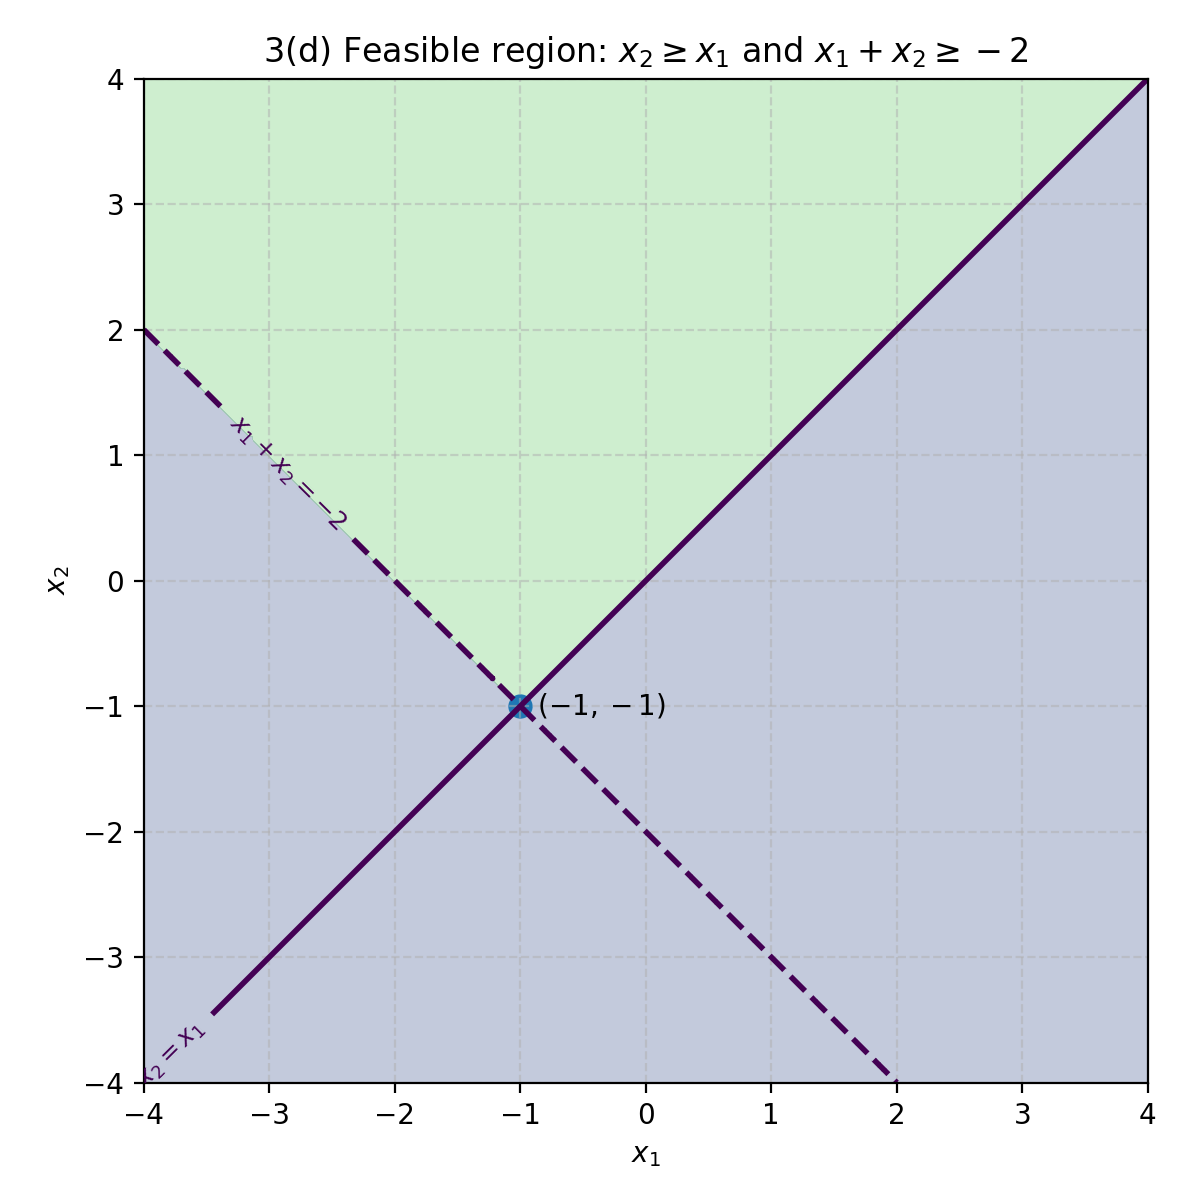
\includegraphics[width=0.6\textwidth]{3d.png}
		\caption{Feasible wedge $x_2\ge x_1$, $x_1+x_2\ge -2$ with corner at $(-1,-1)$.}
	\end{figure}
	
	\item \textbf{Problem statement.}
	Confirm 3(d) with \texttt{scipy.optimize.linprog}.
	
	\emph{Answer (code).}
	\begin{lstlisting}[language=Python]
import numpy as np
from scipy.optimize import linprog

A = np.array([[-1.0, 1.0],
[ 0.5, 0.5]])
b = np.array([0.0, 1.0])
c = np.array([0.0, 2.0])             # minimize c^T x = 2*x2
A_ub = np.array([[ 1.0, -1.0],       # x1 - x2 <= 0   (x2 >= x1)
[-1.0, -1.0]])      # -x1 - x2 <= 2  (x1 + x2 >= -2)
b_ub = np.array([0.0, 2.0])

res = linprog(c, A_ub=A_ub, b_ub=b_ub,
bounds=[(None, None)]*2, method="highs")
y = A @ res.x + b
orig_obj = np.array([1.0, 2.0]) @ y
		
print("status:", res.message)
print("x*     :", res.x)
print("obj c^T x:", res.fun)
print("y      :", y)
print("[1 2]^T y:", orig_obj)
print("y >= 0? ", np.all(y >= -1e-10))
	\end{lstlisting}
	
	\emph{Answer (output).}
	\begin{lstlisting}
status: Optimization terminated successfully. (HiGHS Status 7: Optimal)
x*     : [-1. -1.]
obj c^T x: -2.0
y      : [0. 0.]
[1 2]^T y: 0.0
y >= 0?  True
	\end{lstlisting}
	Thus $x^\star=(-1,-1)$, $y^\star=(0,0)$, and $[1\;2]^T y^\star=0$, matching 3(d).
\end{enumerate}

\newpage
	
\textbf{Problem 4. Basics of the use of the $\ell_1$ norm.}

\begin{enumerate}[label=4(\alph*)]
	
	\item Consider the constraint $\sum_{i=1}^{n}|x_i|\le 1$. Draw the feasible region for $n=2$.
	
	\emph{Answer.}
	For $n=2$, $\{|x_1|+|x_2|\le 1\}$ is a diamond (square at $45^\circ$) with vertices $(1,0),(0,1),(-1,0),(0,-1)$.
	Equivalently it is given by the four halfspaces
	$x_1+x_2\le 1,\ -x_1+x_2\le 1,\ x_1-x_2\le 1,\ -x_1-x_2\le 1$.
	\begin{figure}[H]\centering
		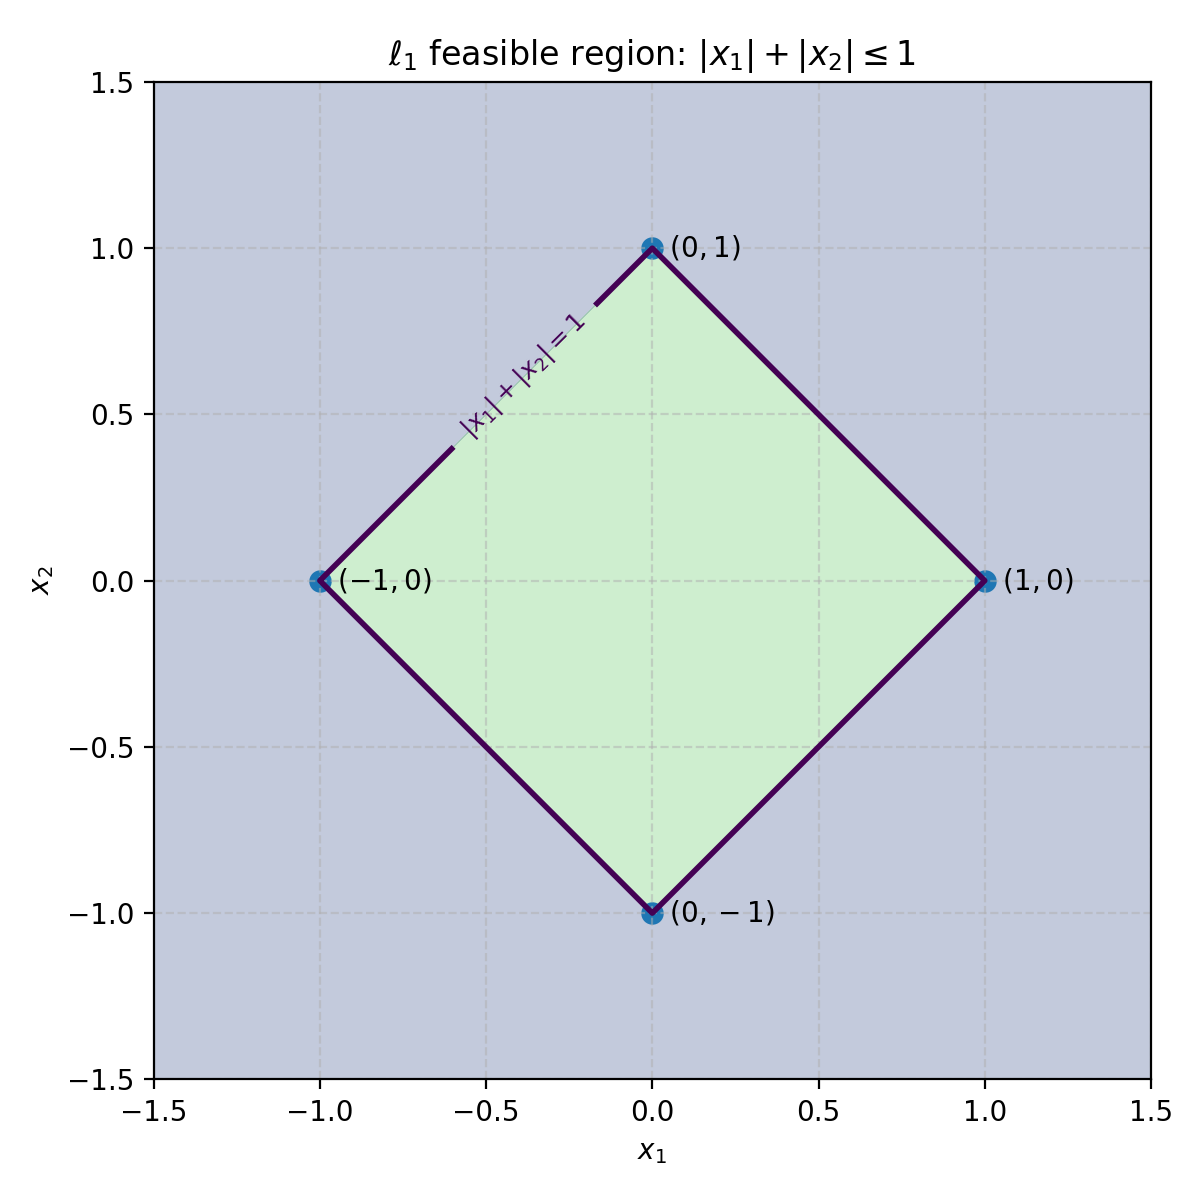
\includegraphics[width=0.45\textwidth]{4a.png}
		\caption{Feasible region for $|x_1|+|x_2|\le 1$ ($\ell_1$ unit ball in $\mathbb{R}^2$).}
	\end{figure}
	
	\item Restate the above inequality in standard form using $c_i(x)$, $i=1,2,3,4$.
	
	\emph{Answer.}
	\[
	\boxed{
		\begin{aligned}
			c_1(x)&=x_1+x_2-1,\\
			c_2(x)&=-x_1+x_2-1,\\
			c_3(x)&=x_1-x_2-1,\\
			c_4(x)&=-x_1-x_2-1,
	\end{aligned}}
	\qquad\text{enforce } c_i(x)\le 0\ (i=1,\dots,4).
	\]
	
	\item Consider the general case $\sum_{i=1}^{n}|x_i|\le M$ with $M<n$ and integer $n$.
	\begin{enumerate}[label=\roman*)]
		\item List the corner points. \quad
		\emph{Answer.} $2n$ corners: $\{\pm M\,e_i\}_{i=1}^n$.
		\item For each corner point, show the count of the nonzero entries. \quad
		\emph{Answer.} Exactly one nonzero entry (equal to $\pm M$).
	\end{enumerate}
	
	\item Restate the inequality using $c_i(x)$ for $n=3$.  
	How many $c_i(x)$ are needed for arbitrary $n$?  
	Why does the $\ell_1$–norm often require constraint approximations?
	
	\emph{Answer.}
	For $n=3$ use all sign patterns:
	\[
	c_{\sigma}(x)=\sigma_1 x_1+\sigma_2 x_2+\sigma_3 x_3 - M \le 0,
	\quad \sigma_i\in\{\pm1\}\ \Rightarrow\ 2^3\ \text{constraints}.
	\]
	In general, $2^n$ constraints are needed; this exponential growth motivates approximate treatments of the $\ell_1$ constraint in practice.
	
\end{enumerate}

\newpage
	
\textbf{Problem 5. Unconstrained optimization.}

Consider the function
\[
f(x_1,x_2) = (x_1 - 2)^2 + 10\,(x_2 - 3)^2.
\]

\begin{enumerate}[label=\arabic*)]
	\item \emph{Contours and gradient.}
	\[
	\nabla f(x)=\begin{bmatrix}2(x_1-2)\\ 20(x_2-3)\end{bmatrix}.
	\]
	Contours and the gradient field are shown in Fig.~\ref{fig:p5}.
	
	\item \emph{Stationary point.}
	Solve $\nabla f(x)=0 \Rightarrow x^\star=(2,3)$.
	
	\item \emph{Unconstrained minimum.}
	The Hessian $\nabla^2 f=\begin{bmatrix}2&0\\0&20\end{bmatrix}\succ0$, so $x^\star$ is the unique global minimizer with $f(x^\star)=0$.
	
	\item \emph{Verification.}
	$\nabla f(x^\star)=\mathbf{0}$ (confirmed numerically below).
\end{enumerate}

\begin{verbatim}
	=== Problem 5 Answers ===
	Analytic stationary point (grad f=0):
	x* (analytic)   = [2, 3]
	grad f(x*) (analytic) = [0, 0]
	f(x*) (analytic) = 0
	H positive definite? True (eigs = [2, 20])
	
	Gradient-descent solution (demonstration):
	x* (GD)         = [2, 5]  (iters <= 200)
	grad f(x*) (GD)     = [0, 40]
	f(x*) (GD)      = 40
\end{verbatim}

\begin{figure}[H]
	\centering
	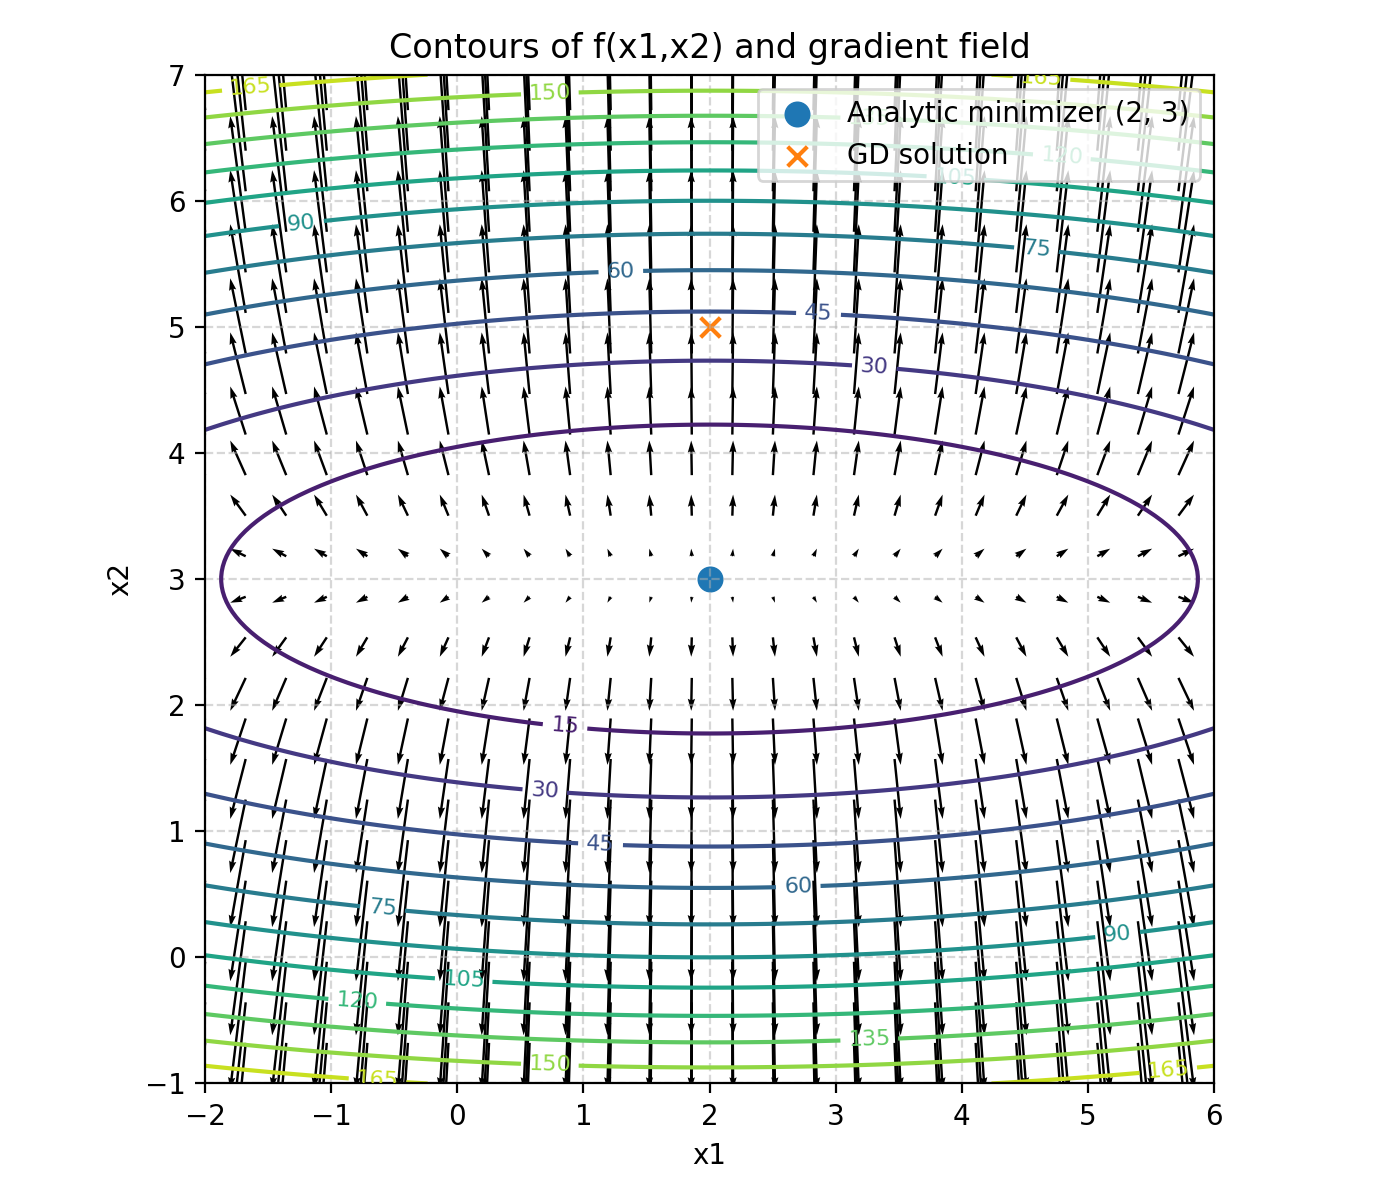
\includegraphics[width=0.52\textwidth]{5.png}
	\caption{Contours of $f(x_1,x_2)$ and gradient field; minimizer at $(2,3)$.}
	\label{fig:p5}
\end{figure}

\newpage

\textbf{Problem 6. Constrained optimization.}

Consider the following ideal, convex optimization problem:
\[
\min_{x}\ f(x_1,x_2) \tag{19}
\]
subject to
\[
\sum_{i=1}^{n} |x_i| \le 1.
\]

\begin{enumerate}[label=6(\alph*)]
	\item Let $f(x_1,x_2)=(x_1-1)^2+(x_2-4)^2$.
	\begin{enumerate}[label=\arabic*)]
		\item Plot the contours of the function and its constraints.
		\item Solve the unconstrained optimization problem:
		\[
		\min_{x}\ f(x_1,x_2). \tag{20}
		\]
		\item Solve the constrained optimization problem by finding the point in the line
		constraint that is closest to the unconstrained optimal point.
	\end{enumerate}

	\textbf{Solution.}
	
	\begin{enumerate}[label=\arabic*)]
		\item \emph{Contours and constraint.} The feasible set is the $\ell_1$ ball
		\[
		|x_1|+|x_2|\le 1,
		\]
		a diamond with vertices $(\pm 1,0)$ and $(0,\pm 1)$. The plot is shown below.
		
		\begin{figure}[H]
			\centering
			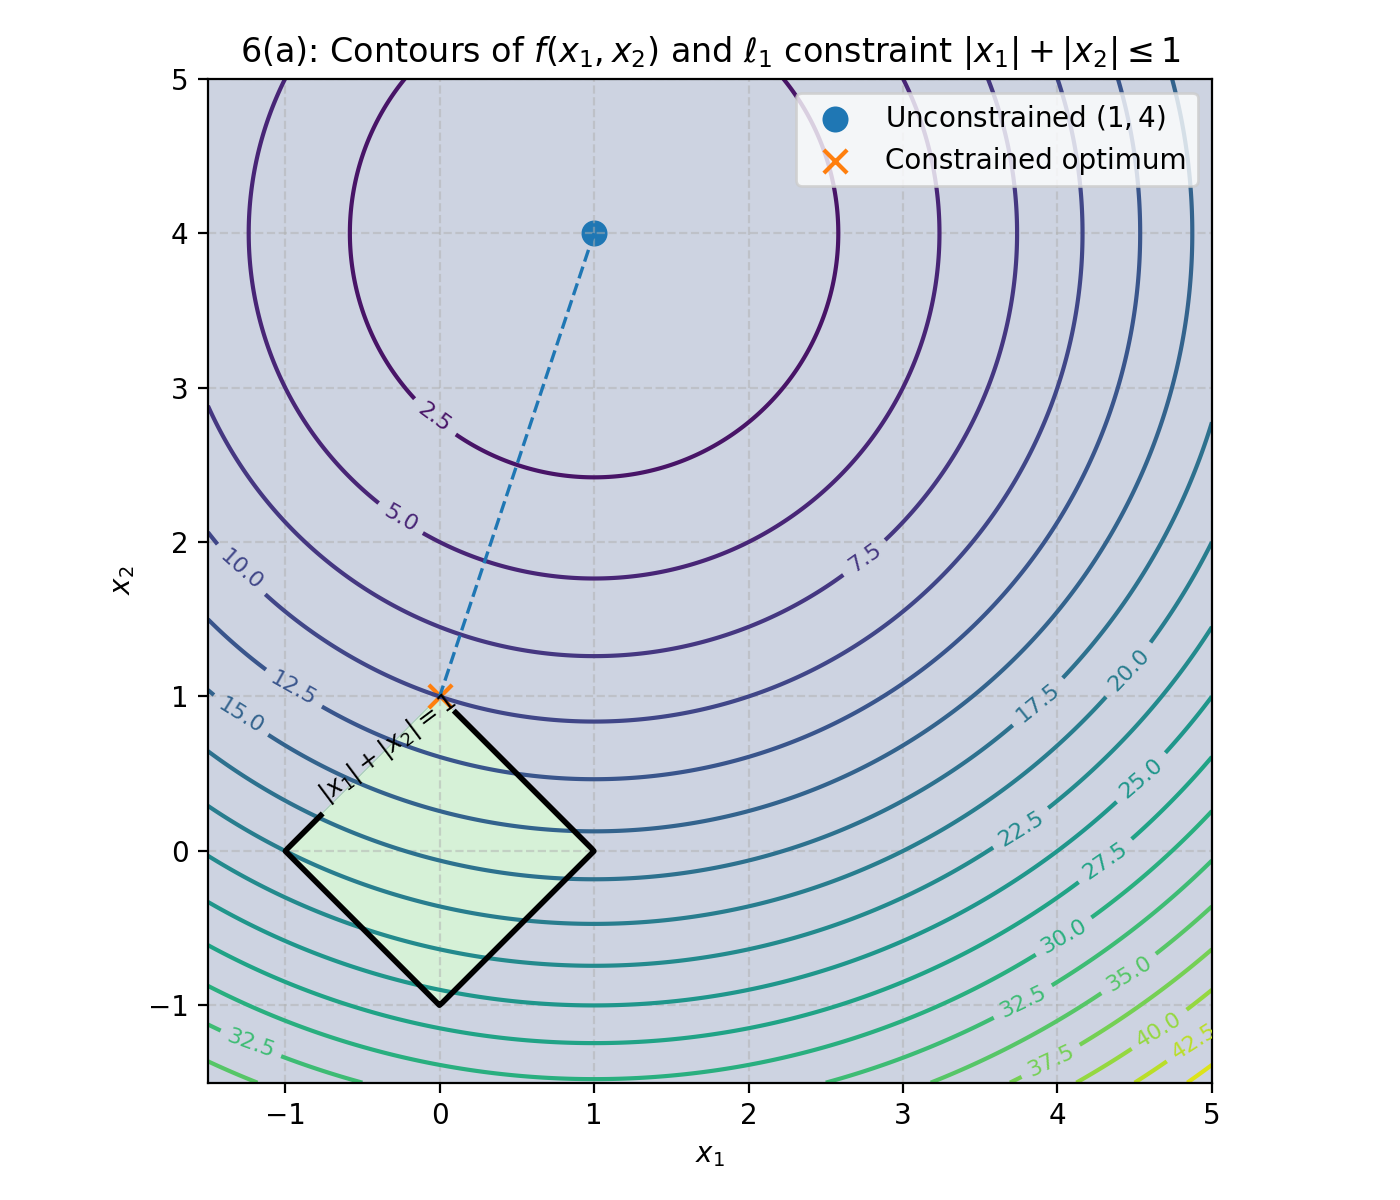
\includegraphics[width=0.55\textwidth]{6a.png}
			\caption{Contours of $f(x_1,x_2)$ and the constraint $|x_1|+|x_2|\le 1$. The unconstrained minimizer $(1,4)$ and the constrained solution $(0,1)$ are marked.}
		\end{figure}
		
		\item \emph{Unconstrained optimum.} 
		\[
		\nabla f(x)=\begin{bmatrix}2(x_1-1)\\ 2(x_2-4)\end{bmatrix}=0
		\ \Rightarrow\ x_u=(1,4),\qquad f(x_u)=0,\qquad \|x_u\|_1=5>1,
		\]
		so $x_u$ is infeasible.
		
		\item \emph{Constrained optimum.} The solution is the point in $|x_1|+|x_2|\le 1$ closest (in Euclidean distance) to $x_u$, i.e., the projection of $(1,4)$ onto the $\ell_1$ ball:
		\[
		x_c=(0,1),\qquad \|x_c\|_1=1\ \text{(on boundary)},\qquad f(x_c)=(0-1)^2+(1-4)^2=10.
		\]
	\end{enumerate}

	\item Let $f(x_1,x_2)=(x_1-5)^2+x_2^2$.
	\begin{enumerate}[label=\arabic*)]
		\item Plot the contours of the function and its constraints.
		\item Solve the unconstrained optimization problem:
		\[
		\min_{x}\ f(x_1,x_2). \tag{21}
		\]
		\item Solve the constrained optimization problem by finding the point that is
		closest to the unconstrained optimal point.
	\end{enumerate}
	
	\textbf{Solution.}
	
	\begin{enumerate}[label=\arabic*)]
		\item \emph{Contours and constraint.} The feasible set is the $\ell_1$ ball
		\[
		|x_1|+|x_2|\le 1,
		\]
		a diamond with vertices $(\pm 1,0)$ and $(0,\pm 1)$. The plot is shown below.
		
		\begin{figure}[H]
			\centering
			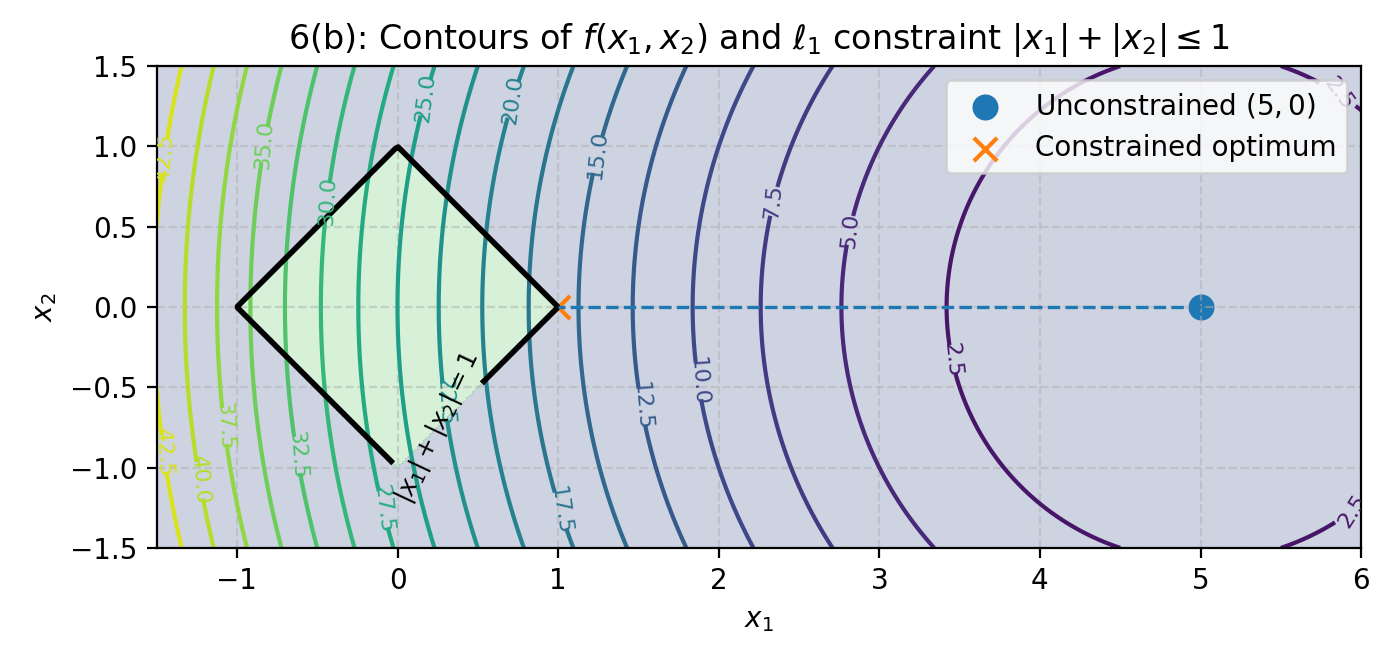
\includegraphics[width=0.55\textwidth]{6b.png}
			\caption{Contours of $f(x_1,x_2)=(x_1-5)^2+x_2^2$ and the constraint $|x_1|+|x_2|\le 1$. The unconstrained minimizer $(5,0)$ and the constrained solution $(1,0)$ are marked.}
		\end{figure}
		
		\item \emph{Unconstrained optimum.}
		\[
		\nabla f(x)=\begin{bmatrix}2(x_1-5)\\ 2x_2\end{bmatrix}=0
		\ \Rightarrow\ x_u=(5,0),\qquad f(x_u)=0,\qquad \|x_u\|_1=5>1,
		\]
		so $x_u$ is infeasible.
		
		\item \emph{Constrained optimum.} The solution is the point in $|x_1|+|x_2|\le 1$ closest (in Euclidean distance) to $x_u$, i.e., the projection of $(5,0)$ onto the $\ell_1$ ball:
		\[
		x_c=(1,0),\qquad \|x_c\|_1=1\ \text{(on boundary)},\qquad f(x_c)=(1-5)^2+0^2=16.
		\]
	\end{enumerate}
	
	\item Let $f(x_1,x_2)=(x_1-0.5)^2+x_2^2$.
	\begin{enumerate}[label=\arabic*)]
		\item Plot the contours of the function and its constraints.
		\item Solve the unconstrained optimization problem:
		\[
		\min_{x}\ f(x_1,x_2).
		\]
		\item Based on your contour plot, show that the optimal point cannot be on the
		boundary.
	\end{enumerate}
	
	\textbf{Solution.}
	
	\begin{enumerate}[label=\arabic*)]
		\item \emph{Contours and constraint.} The feasible set is the $\ell_1$ ball
		\[
		|x_1|+|x_2|\le 1,
		\]
		a diamond with vertices $(\pm 1,0)$ and $(0,\pm 1)$. The plot is shown below.
		
		\begin{figure}[H]
			\centering
			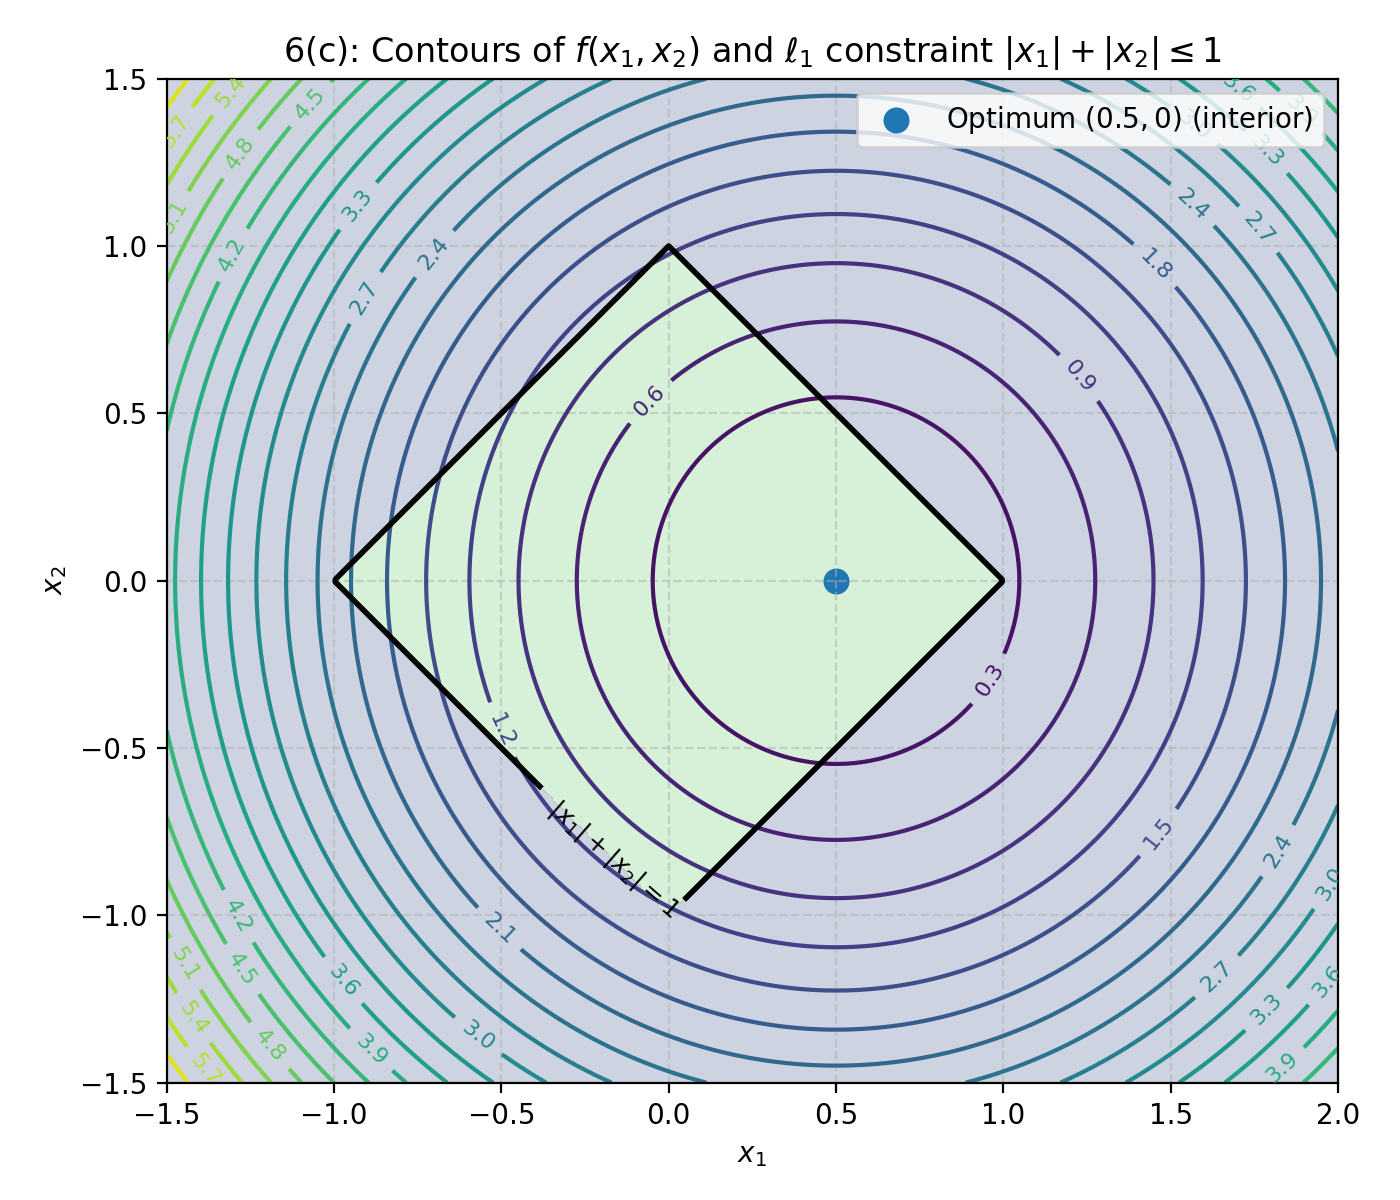
\includegraphics[width=0.55\textwidth]{6c.png}
			\caption{Contours of $f(x_1,x_2)=(x_1-0.5)^2+x_2^2$ and the constraint $|x_1|+|x_2|\le 1$. The point $(0.5,0)$ is marked and lies strictly inside the feasible diamond.}
		\end{figure}
		
		\item \emph{Unconstrained optimum.}
		\[
		\nabla f(x)=\begin{bmatrix}2(x_1-0.5)\\ 2x_2\end{bmatrix}=0
		\ \Rightarrow\ x_u=(0.5,0),\quad f(x_u)=0,\quad \|x_u\|_1=0.5<1,
		\]
		so $x_u$ is feasible and in the interior.
		
		\item \emph{Not on the boundary.} Since the unconstrained minimizer is feasible and strictly interior, the constrained optimum coincides with it:
		\[
		x_c=(0.5,0),\qquad f(x_c)=0,
		\]
		hence the optimal point cannot be on the boundary.
	\end{enumerate}
	
	\item Verify that the KKT conditions are satisfied at the optimal points for
	6(a), 6(b), and 6(c).
	
	\textbf{Solution.}
	
	Use inequality form $c_i(x)\le 0$ for the $\ell_1$ ball in $\mathbb{R}^2$:
	\[
	c_1=x_1+x_2-1,\;\; c_2=-x_1+x_2-1,\;\; c_3=x_1-x_2-1,\;\; c_4=-x_1-x_2-1,
	\]
	and Lagrangian \(L(x,\lambda)=f(x)+\sum_i\lambda_i c_i(x)\), \(\lambda_i\ge 0\).
	
	\begin{enumerate}[label=\arabic*)]
		\item \emph{6(a)} \(f=(x_1-1)^2+(x_2-4)^2,\; x^\star=(0,1)\).  
		Active: \(c_1=c_2=0\).  
		\[
		\nabla f(x^\star)=\begin{bmatrix}-2\\-6\end{bmatrix},\quad
		\nabla c_1=\begin{bmatrix}1\\1\end{bmatrix},\;
		\nabla c_2=\begin{bmatrix}-1\\1\end{bmatrix}.
		\]
		Stationarity \(\nabla f+\lambda_1\nabla c_1+\lambda_2\nabla c_2=0\Rightarrow
		\lambda_1=4,\;\lambda_2=2\ (\ge0).\)  
		CS holds, LICQ: \(\det\!\begin{bmatrix}1&-1\\1&1\end{bmatrix}=2\neq0\). KKT satisfied.
		
		\item \emph{6(b)} \(f=(x_1-5)^2+x_2^2,\; x^\star=(1,0)\).  
		Active: \(c_1=c_3=0\).  
		\[
		\nabla f(x^\star)=\begin{bmatrix}-8\\0\end{bmatrix},\quad
		\nabla c_1=\begin{bmatrix}1\\1\end{bmatrix},\;
		\nabla c_3=\begin{bmatrix}1\\-1\end{bmatrix}.
		\]
		Stationarity \(\Rightarrow \lambda_1=\lambda_3=4\ (\ge0)\).  
		CS holds, LICQ: \(\det\!\begin{bmatrix}1&1\\1&-1\end{bmatrix}=-2\neq0\). KKT satisfied.
		
		\item \emph{6(c)} \(f=(x_1-0.5)^2+x_2^2,\; x^\star=(0.5,0)\) is interior (\(\|x^\star\|_1=0.5<1\)).  
		No active constraints, \(\nabla f(x^\star)=0,\ \lambda=0\). KKT satisfied.
	\end{enumerate}
	
	\medskip
	\noindent\textbf{KKT Summary.}
	In constrained optimization, the KKT conditions are always satisfied at the optimal point. Note that this is not enough to determine if a point is optimal. If the KKT conditions are satisfied, we cannot infer that we have an optimal point. To understand the KKT conditions, we need to apply them. Here is an intuitive summary of how to apply and verify the KKT conditions:
	
	\begin{itemize}
		\item \textbf{IF} the solution is at an interior point, \textbf{THEN} the gradient of $f$ should be zero at that point.
		\item \textbf{IF} the solution is on a boundary point and LICQ holds there, \textbf{THEN} the Lagrangian condition is satisfied at that point.
	\end{itemize}
	
	To understand the KKT conditions, note that they only tell you when you can reject a candidate optimal point. For a contra-positive: Suppose we have “IF A THEN B.” The equivalent statement is “IF (NOT B) THEN (NOT A).” Since A implies B, if B does not hold, then A does not hold either. Applying this:
	
	\begin{itemize}
		\item If the gradient of $f$ is not zero in the interior, we can conclude the optimal solution is not in the interior.
		\item If the Lagrangian condition is not satisfied, then either the solution is not on the boundary or LICQ does not hold.
	\end{itemize}
	
	If the KKT conditions are satisfied, then we \emph{may} be at an optimal point. There are no guarantees that we will be optimal. If A implies B, we cannot say that B implies A.
	
	Next, we explain each condition. For the first condition, if $x^*$ is inside the feasible region, we require that $\nabla f(x^*)=0$. Again, this is not enough to guarantee optimality. However, if this condition is violated, we are clearly not at an optimal point in the interior.
	
	If the solution is not inside the feasible region, then it could be on the boundary of the feasible region. In this case, we need to first check the LICQ condition before we look at the full KKT conditions.
	
	For the LICQ condition, consider the vectors evaluated at the candidate optimal point. Here, we are only concerned with the constraints that are active (those satisfying $c_i(x^*)=0$). Thus, if a solution is on a line, the $c_i(x)$ that gives the equation of the line will satisfy $c_i(x^*)=0$. For a corner, we will have $c_i(x^*)=c_j(x^*)=0$ for the two intersecting lines. LICQ requires that $\{\nabla c_i(x^*)\}_{i\in\mathcal{A}}$ are linearly independent, i.e.,
	\[
	\sum_{\text{Active } i} a_i\,\nabla c_i(x^*)=0 \quad\Longrightarrow\quad a_i=0\ \ \text{for all $i$.} \tag{23}
	\]
	
	To check the Lagrangian condition, form the Lagrangian
	\[
	L(x,\lambda)=f(x)-\sum_{\text{Active } i}\lambda_i\,c_i(x). \tag{24}
	\]
	The Lagrangian condition requires that we can solve
	\[
	\nabla_x L(x^*,\lambda^*)=0 \tag{25}
	\]
	at the optimal point $x^*$ for some $\lambda_i^*\ge 0$. It is important to understand what (25) is saying: basically, it says that going inside the feasible region will only increase the function. Note that $\nabla f$ is the direction where the function is increasing. Furthermore, (25) implies
	\[
	\nabla f(x^*)-\sum_{\text{Active } i}\lambda_i^*\,\nabla c_i(x^*)=0, \tag{26}
	\]
	which can be rewritten as
	\[
	-\nabla f(x^*)=-\sum_{\text{Active } i}\lambda_i^*\,\nabla c_i(x^*). \tag{27}
	\]
	Thus, the descent direction $-\nabla f(x^*)$ points outside the feasible region.
\end{enumerate}

\medskip
\noindent\textbf{Contour and gradient plots in Python.}
For information on how to plot contours, the following links can help a lot:
\begin{itemize}
	\item A simple unofficial tutorial on how to generate contours in Python: \url{https://www.python-course.eu/matplotlib_contour_plot.php}.
	\item The official tutorial of how to plot 2D contours from regularly-spaced points.
	\item The official tutorial of how to plot 2D contours from irregularly-spaced points (needed later).
	\item An official advanced tutorial for using advanced options for contour plots can be found at the advanced contour tutorial.
	\item An official simple demo of how to use quiver to plot gradient fields.
	\item In Matplotlib, you can plot the contours followed by the gradient and they will appear together (equivalent to having \texttt{hold on} as the default behavior).
\end{itemize}

\noindent\textbf{Advanced Demo for Optimization Methods in Python.}
You can find a very nice demonstration of how to produce convergence videos of several unconstrained optimization algorithms.

\newpage

\section{Appendix: Code}
\begin{lstlisting}
import sys
import numpy as np
import matplotlib.pyplot as plt
from scipy.optimize import linprog

sys.stdout.reconfigure(encoding="utf-8")
def fmt(x): return f"{float(x):.2g}"
def fmt_vec(v): return "[" + ", ".join(fmt(t) for t in np.atleast_1d(v)) + "]"

# --- Plot helpers (consistent style across problems) ---
def setup_square(xmin, xmax, ymin, ymax, title="", xlabel=r"$x_1$", ylabel=r"$x_2$"):
plt.figure(figsize=(6, 6))
if title:
plt.title(title)
plt.xlabel(xlabel)
plt.ylabel(ylabel)
plt.xlim(xmin, xmax)
plt.ylim(ymin, ymax)
plt.gca().set_aspect("equal", adjustable="box")
plt.grid(True, linestyle="--", alpha=0.5)

def save_png(name):
plt.tight_layout()
plt.savefig(name, dpi=200)

# =========================
# Problem 1(c)
# =========================
def problem_1c():
# Feasible region: x1 >= 0, x2 >= 0, x1 + 2 x2 <= 2 (triangle with (0,0),(2,0),(0,1))
setup_square(
0, 2.1, 0, 1.1,
title=r"Feasible region for $x_1\geq 0,\ x_2\geq 0,\ x_1+2x_2\leq 2$"
)
# Shade feasible polygon
plt.fill([0, 2, 0], [0, 0, 1], color="lightblue", alpha=0.5, label="Feasible region")
# Boundary line x1 + 2 x2 = 2 (endpoints)
plt.plot([2, 0], [0, 1], linewidth=2, label=r"$x_1+2x_2=2$")
plt.scatter([2, 0], [0, 1], s=60)
plt.text(2, 0, r"  $(2,0)$", va="center")
plt.text(0, 1, r"  $(0,1)$", va="center")
plt.legend(loc="upper right")
save_png("1c.png")

# =========================
# Problem 3(c)
# =========================
def problem_3c():
# s(x) = c^T ReLU(Ax+b)
A = np.array([[-1.0,  1.0],
[ 0.5,  0.5]])
b = np.array([0.0, 1.0])
c = np.array([1.0, 2.0])

x1_min, x1_max = -2.0, 2.0
x2_min, x2_max = -2.0, 2.0
res = 400
x1 = np.linspace(x1_min, x1_max, res)
x2 = np.linspace(x2_min, x2_max, res)
X1, X2 = np.meshgrid(x1, x2)
P = np.stack([X1.ravel(), X2.ravel()], axis=1)

H = (P @ A.T) + b       # pre-activations
Y = np.maximum(0.0, H)  # ReLU
S = (Y @ c).reshape(res, res)
H_maps = [H[:, i].reshape(res, res) for i in range(A.shape[0])]

# (i) Hidden-region boundaries and active sides
setup_square(x1_min, x1_max, x2_min, x2_max,
title=r"Hidden regions: $a_i^{\top}x+b_i=0$ and active sides (ReLU)")
for i, H_i in enumerate(H_maps):
plt.contourf(X1, X2, (H_i > 0).astype(float), levels=[-0.5, 0.5, 1.5], alpha=0.15)
cs = plt.contour(X1, X2, H_i, levels=[0.0], linewidths=2)
if cs.allsegs[0]:
plt.clabel(cs, fmt={0.0: f"h_{i+1}=0"}, inline=True, fontsize=9)
save_png("3c_i.png")

# (ii) Output surface s(x) heatmap + contours, with hidden boundaries overlaid
plt.figure(figsize=(7, 6))
plt.title(r"Output surface $s(x)=c^{\top}\mathrm{ReLU}(Ax+b)$")
im = plt.imshow(S, extent=[x1_min, x1_max, x2_min, x2_max],
origin="lower", aspect="equal")
plt.colorbar(im, label=r"$s(x)$")
CS = plt.contour(X1, X2, S, colors="k", linewidths=0.8, levels=10)
plt.clabel(CS, inline=True, fontsize=8, fmt="%.2f")
for H_i in H_maps:
plt.contour(X1, X2, H_i, levels=[0.0], colors="white", linewidths=1.2, alpha=0.9)
plt.xlabel(r"$x_1$")
plt.ylabel(r"$x_2$")
plt.xlim(x1_min, x1_max)
plt.ylim(x2_min, x2_max)
plt.grid(True, linestyle="--", alpha=0.4)
plt.tight_layout()
plt.savefig("3c_ii.png", dpi=200)

# =========================
# Problem 3(d)
# =========================
def problem_3d():
A = np.array([[-1.0,  1.0],
[ 0.5,  0.5]])
b = np.array([0.0, 1.0])

x1_min, x1_max = -4.0, 4.0
x2_min, x2_max = -4.0, 4.0
res = 401
x1 = np.linspace(x1_min, x1_max, res)
x2 = np.linspace(x2_min, x2_max, res)
X1, X2 = np.meshgrid(x1, x2)

Y1 = -X1 + X2 + b[0]           # y1 >= 0 -> x2 >= x1
Y2 = 0.5*X1 + 0.5*X2 + b[1]    # y2 >= 0 -> x1 + x2 >= -2

feasible = (Y1 >= 0) & (Y2 >= 0)

setup_square(x1_min, x1_max, x2_min, x2_max,
title=r"3(d) Feasible region: $x_2\geq x_1$ and $x_1+x_2\geq -2$")
plt.contourf(X1, X2, feasible.astype(float), levels=[-0.5, 0.5, 1.5], alpha=0.3)
C1 = plt.contour(X1, X2, Y1, levels=[0.0], linewidths=2)
C2 = plt.contour(X1, X2, Y2, levels=[0.0], linewidths=2, linestyles="--")
if C1.allsegs[0]:
plt.clabel(C1, fmt={0.0: r"$x_2=x_1$"}, inline=True, fontsize=9)
if C2.allsegs[0]:
plt.clabel(C2, fmt={0.0: r"$x_1+x_2=-2$"}, inline=True, fontsize=9)
corner = (-1.0, -1.0)
plt.scatter([corner[0]], [corner[1]], s=60)
plt.text(corner[0], corner[1], r"  $(-1,-1)$", va="center")
save_png("3d.png")

# =========================
# Problem 3(e)
# =========================
def problem_3e():
# Minimize [0,2]·x s.t. x1 - x2 <= 0, -x1 - x2 <= 2
A_ub = np.array([[ 1.0, -1.0],
[-1.0, -1.0]])
b_ub = np.array([0.0, 2.0])
c = np.array([0.0, 2.0])
bounds = [(None, None), (None, None)]

res = linprog(c, A_ub=A_ub, b_ub=b_ub, bounds=bounds, method="highs")
A = np.array([[-1.0,  1.0],
[ 0.5,  0.5]])
b = np.array([0.0, 1.0])
y = A @ res.x + b
orig_obj = np.array([1.0, 2.0]) @ y

print("=== Problem 3(e) Answers ===")
print(f"status: {res.message}")
print(f"x*     : {fmt_vec(res.x)}")
print(f"obj c^T x: {fmt(res.fun)}")
print(f"y      : {fmt_vec(y)}")
print(f"[1 2]^T y: {fmt(orig_obj)}")
print(f"y >= 0?  {np.all(y >= -1e-10)}")

# =========================
# Problem 4(a)
# =========================
def problem_4a():
x1_min, x1_max = -1.5, 1.5
x2_min, x2_max = -1.5, 1.5
res = 801
x1 = np.linspace(x1_min, x1_max, res)
x2 = np.linspace(x2_min, x2_max, res)
X1, X2 = np.meshgrid(x1, x2)

L1 = np.abs(X1) + np.abs(X2)
feasible = (L1 <= 1.0)

setup_square(x1_min, x1_max, x2_min, x2_max,
title=r"$\ell_1$ feasible region: $|x_1|+|x_2|\leq 1$")
plt.contourf(X1, X2, feasible.astype(float), levels=[-0.5, 0.5, 1.5], alpha=0.30)
C = plt.contour(X1, X2, L1, levels=[1.0], linewidths=2)
if C.allsegs[0]:
plt.clabel(C, fmt={1.0: r"$|x_1|+|x_2|=1$"}, inline=True, fontsize=9)

verts = np.array([[ 1, 0], [ 0, 1], [-1, 0], [ 0,-1]])
labels = [r"$(1,0)$", r"$(0,1)$", r"$(-1,0)$", r"$(0,-1)$"]
plt.scatter(verts[:, 0], verts[:, 1], s=50)
for (xv, yv), lab in zip(verts, labels):
plt.text(xv, yv, "  " + lab, va="center", ha="left")
save_png("4a.png")

# =========================
# Problem 5
# =========================
def problem_5():
def f(x): x1, x2 = x; return (x1 - 2.0)**2 + 10.0*(x2 - 3.0)**2
def grad_f(x): x1, x2 = x; return np.array([2.0*(x1 - 2.0), 20.0*(x2 - 3.0)])
H = np.array([[2.0, 0.0], [0.0, 20.0]])

x_star_analytic = np.array([2.0, 3.0])
grad_at_star = grad_f(x_star_analytic)
f_at_star = f(x_star_analytic)
eigvals = np.linalg.eigvalsh(H)
is_pd = np.all(eigvals > 0)

# Simple GD (demo)
x = np.array([-3.0, 5.0]); alpha = 0.1; max_iters = 200; tol = 1e-10
for k in range(max_iters):
g = grad_f(x)
if np.linalg.norm(g) < tol: break
x -= alpha * g
x_star_gd = x; f_star_gd = f(x_star_gd); grad_at_gd = grad_f(x_star_gd)

print("=== Problem 5 Answers ===")
print("Analytic stationary point (∇f = 0):")
print(f"x* (analytic)       = {fmt_vec(x_star_analytic)}")
print(f"∇f(x*) (analytic)   = {fmt_vec(grad_at_star)}")
print(f"f(x*) (analytic)    = {fmt(f_at_star)}")
print(f"H PD? {is_pd} (eigs = {fmt_vec(eigvals)})\n")
print("Gradient-descent solution (demo):")
print(f"x* (GD)             = {fmt_vec(x_star_gd)}  (iters <= {k+1})")
print(f"∇f(x*) (GD)         = {fmt_vec(grad_at_gd)}")
print(f"f(x*) (GD)          = {fmt(f_star_gd)}")

# Contours + gradient field
x1 = np.linspace(-2.0, 6.0, 200)
x2 = np.linspace(-1.0, 7.0, 200)
X1, X2 = np.meshgrid(x1, x2)
Z = (X1 - 2.0)**2 + 10.0*(X2 - 3.0)**2

skip = 8
X1s, X2s = X1[::skip, ::skip], X2[::skip, ::skip]
U, V = 2.0*(X1s - 2.0), 20.0*(X2s - 3.0)

plt.figure(figsize=(7, 6))
cs = plt.contour(X1, X2, Z, levels=15)
plt.clabel(cs, inline=True, fontsize=8)
plt.quiver(X1s, X2s, U, V, angles="xy", scale_units="xy", scale=60)
plt.scatter([x_star_analytic[0]], [x_star_analytic[1]], s=70, marker="o",
label="Analytic minimizer (2, 3)")
plt.scatter([x_star_gd[0]], [x_star_gd[1]], s=50, marker="x", label="GD solution")
plt.title("Contours of f(x1,x2) and gradient field")
plt.xlabel("x1"); plt.ylabel("x2")
plt.xlim(x1.min(), x1.max()); plt.ylim(x2.min(), x2.max())
plt.gca().set_aspect("equal", adjustable="box")
plt.grid(True, linestyle="--", alpha=0.5)
plt.legend(loc="upper right")
plt.tight_layout()
plt.savefig("5.png", dpi=200)

def problem_6a():
# -------- Problem 6(a): f(x1,x2) = (x1 - 1)^2 + (x2 - 4)^2 --------

# Two-sig-fig formatting (consistent with other problems)
def fmt(x): return f"{float(x):.2g}"
def fmt_vec(v): return "[" + ", ".join(fmt(t) for t in np.atleast_1d(v)) + "]"

# Objective
def f(x):
x1, x2 = x
return (x1 - 1.0)**2 + (x2 - 4.0)**2

# Euclidean projection onto the l1 ball of radius 1
def project_onto_l1(u, radius=1.0):
u = np.asarray(u, dtype=float)
if np.sum(np.abs(u)) <= radius:
return u.copy()
a = np.abs(u)
s = np.sort(a)[::-1]
cssv = np.cumsum(s)
rho = np.max(np.where(s - (cssv - radius) / (np.arange(1, len(s)+1)) > 0)[0]) + 1
tau = (cssv[rho-1] - radius) / rho
return np.sign(u) * np.maximum(a - tau, 0.0)

# Unconstrained minimizer: ∇f=0 -> (1,4)
x_u = np.array([1.0, 4.0])

# Constrained minimizer: projection of x_u onto |x1|+|x2| <= 1
x_c = project_onto_l1(x_u, radius=1.0)

# Print answers
print("=== Problem 6(a) Answers ===")
print("Unconstrained minimizer:")
print(f"x_u          = {fmt_vec(x_u)}")
print(f"f(x_u)       = {fmt(f(x_u))}")
print(f"||x_u||_1    = {fmt(np.sum(np.abs(x_u)))}")
print("\nConstrained minimizer (projection onto |x1|+|x2|<=1):")
print(f"x_c          = {fmt_vec(x_c)}")
print(f"f(x_c)       = {fmt(f(x_c))}")
print(f"||x_c||_1    = {fmt(np.sum(np.abs(x_c)))}  (should be 1 if on boundary)")

# -------- Plot: contours + l1 constraint + points --------
x1_min, x1_max = -1.5, 5.0
x2_min, x2_max = -1.5, 5.0
res = 400
x1 = np.linspace(x1_min, x1_max, res)
x2 = np.linspace(x2_min, x2_max, res)
X1, X2 = np.meshgrid(x1, x2)

Z  = (X1 - 1.0)**2 + (X2 - 4.0)**2                          # f(x)
L1 = np.abs(X1) + np.abs(X2)                                # |x1|+|x2|
feasible = (L1 <= 1.0)

plt.figure(figsize=(7, 6))
plt.title(r"6(a): Contours of $f(x_1,x_2)$ and $\ell_1$ constraint $|x_1|+|x_2|\leq 1$")

# Contours of f
cs = plt.contour(X1, X2, Z, levels=20)
plt.clabel(cs, inline=True, fontsize=8)

# Shade feasible l1 region and draw boundary
plt.contourf(X1, X2, feasible.astype(float), levels=[-0.5, 0.5, 1.5], alpha=0.25)
C = plt.contour(X1, X2, L1, levels=[1.0], colors='k', linewidths=2)
if C.allsegs[0]:
plt.clabel(C, fmt={1.0: r"$|x_1|+|x_2|=1$"}, inline=True, fontsize=9)

# Mark points and projection segment
plt.scatter([x_u[0]], [x_u[1]], s=70, marker='o', label=r'Unconstrained $(1,4)$')
plt.scatter([x_c[0]], [x_c[1]], s=70, marker='x', label='Constrained optimum')
plt.plot([x_u[0], x_c[0]], [x_u[1], x_c[1]], linestyle='--', linewidth=1.2)

plt.xlabel(r"$x_1$")
plt.ylabel(r"$x_2$")
plt.xlim(x1_min, x1_max)
plt.ylim(x2_min, x2_max)
plt.gca().set_aspect('equal', adjustable='box')
plt.grid(True, linestyle='--', alpha=0.5)
plt.legend(loc='upper right')
plt.tight_layout()
plt.savefig("6a.png", dpi=200)

def problem_6b():
# -------- Problem 6(b): f(x1,x2) = (x1 - 5)^2 + x2^2 --------

# Two-sig-fig formatting
def fmt(x): return f"{float(x):.2g}"
def fmt_vec(v): return "[" + ", ".join(fmt(t) for t in np.atleast_1d(v)) + "]"

# Objective
def f(x):
x1, x2 = x
return (x1 - 5.0)**2 + (x2 - 0.0)**2

# Euclidean projection onto the l1 ball of radius 1
def project_onto_l1(u, radius=1.0):
u = np.asarray(u, dtype=float)
if np.sum(np.abs(u)) <= radius:
return u.copy()
a = np.abs(u)
s = np.sort(a)[::-1]
cssv = np.cumsum(s)
rho = np.max(np.where(s - (cssv - radius) / (np.arange(1, len(s)+1)) > 0)[0]) + 1
tau = (cssv[rho-1] - radius) / rho
return np.sign(u) * np.maximum(a - tau, 0.0)

# Unconstrained minimizer: ∇f=0 -> (5,0)
x_u = np.array([5.0, 0.0])

# Constrained minimizer: projection of x_u onto |x1|+|x2| <= 1
x_c = project_onto_l1(x_u, radius=1.0)

# Print answers
print("=== Problem 6(b) Answers ===")
print("Unconstrained minimizer:")
print(f"x_u          = {fmt_vec(x_u)}")
print(f"f(x_u)       = {fmt(f(x_u))}")
print(f"||x_u||_1    = {fmt(np.sum(np.abs(x_u)))}")
print("\nConstrained minimizer (projection onto |x1|+|x2|<=1):")
print(f"x_c          = {fmt_vec(x_c)}")
print(f"f(x_c)       = {fmt(f(x_c))}")
print(f"||x_c||_1    = {fmt(np.sum(np.abs(x_c)))}  (should be 1 if on boundary)")

# -------- Plot: contours + l1 constraint + points --------
x1_min, x1_max = -1.5, 6.0
x2_min, x2_max = -1.5, 1.5
res = 400
x1 = np.linspace(x1_min, x1_max, res)
x2 = np.linspace(x2_min, x2_max, res)
X1, X2 = np.meshgrid(x1, x2)

Z  = (X1 - 5.0)**2 + (X2 - 0.0)**2                     # f(x)
L1 = np.abs(X1) + np.abs(X2)                            # |x1|+|x2|
feasible = (L1 <= 1.0)

plt.figure(figsize=(7, 6))
plt.title(r"6(b): Contours of $f(x_1,x_2)$ and $\ell_1$ constraint $|x_1|+|x_2|\leq 1$")

# Contours of f
cs = plt.contour(X1, X2, Z, levels=20)
plt.clabel(cs, inline=True, fontsize=8)

# Shade feasible l1 region and draw boundary
plt.contourf(X1, X2, feasible.astype(float), levels=[-0.5, 0.5, 1.5], alpha=0.25)
C = plt.contour(X1, X2, L1, levels=[1.0], colors='k', linewidths=2)
if C.allsegs[0]:
plt.clabel(C, fmt={1.0: r"$|x_1|+|x_2|=1$"}, inline=True, fontsize=9)

# Mark points and projection segment
plt.scatter([x_u[0]], [x_u[1]], s=70, marker='o', label=r'Unconstrained $(5,0)$')
plt.scatter([x_c[0]], [x_c[1]], s=70, marker='x', label='Constrained optimum')
plt.plot([x_u[0], x_c[0]], [x_u[1], x_c[1]], linestyle='--', linewidth=1.2)

plt.xlabel(r"$x_1$")
plt.ylabel(r"$x_2$")
plt.xlim(x1_min, x1_max)
plt.ylim(x2_min, x2_max)
plt.gca().set_aspect('equal', adjustable='box')
plt.grid(True, linestyle='--', alpha=0.5)
plt.legend(loc='upper right')
plt.tight_layout()
plt.savefig("6b.png", dpi=200)

def problem_6c():
# -------- Problem 6(c): f(x1,x2) = (x1 - 0.5)^2 + x2^2 --------

# Two-sig-fig formatting
def fmt(x): return f"{float(x):.2g}"
def fmt_vec(v): return "[" + ", ".join(fmt(t) for t in np.atleast_1d(v)) + "]"

# Objective
def f(x):
x1, x2 = x
return (x1 - 0.5)**2 + (x2 - 0.0)**2

# Unconstrained minimizer: ∇f=0 -> (0.5, 0)
x_u = np.array([0.5, 0.0])
l1_u = np.sum(np.abs(x_u))
on_boundary = np.isclose(l1_u, 1.0, atol=1e-12)

# Since ||x_u||_1 = 0.5 < 1, the constrained optimum equals x_u (interior point)
x_c = x_u.copy()

# Print answers
print("=== Problem 6(c) Answers ===")
print("Unconstrained minimizer:")
print(f"x_u          = {fmt_vec(x_u)}")
print(f"f(x_u)       = {fmt(f(x_u))}")
print(f"||x_u||_1    = {fmt(l1_u)}  (<= 1, interior)")
print("\nConstrained minimizer:")
print(f"x_c          = {fmt_vec(x_c)}  (same as x_u; interior)")
print(f"f(x_c)       = {fmt(f(x_c))}")
print(f"on boundary? = {on_boundary}")

# -------- Plot: contours + l1 constraint + point --------
x1_min, x1_max = -1.5, 2.0
x2_min, x2_max = -1.5, 1.5
res = 400
x1 = np.linspace(x1_min, x1_max, res)
x2 = np.linspace(x2_min, x2_max, res)
X1, X2 = np.meshgrid(x1, x2)

Z  = (X1 - 0.5)**2 + (X2 - 0.0)**2                 # f(x)
L1 = np.abs(X1) + np.abs(X2)                        # |x1|+|x2|
feasible = (L1 <= 1.0)

plt.figure(figsize=(7, 6))
plt.title(r"6(c): Contours of $f(x_1,x_2)$ and $\ell_1$ constraint $|x_1|+|x_2|\leq 1$")

# Contours of f
cs = plt.contour(X1, X2, Z, levels=20)
plt.clabel(cs, inline=True, fontsize=8)

# Shade feasible l1 region and draw boundary
plt.contourf(X1, X2, feasible.astype(float), levels=[-0.5, 0.5, 1.5], alpha=0.25)
C = plt.contour(X1, X2, L1, levels=[1.0], colors='k', linewidths=2)
if C.allsegs[0]:
plt.clabel(C, fmt={1.0: r"$|x_1|+|x_2|=1$"}, inline=True, fontsize=9)

# Mark interior optimum
plt.scatter([x_u[0]], [x_u[1]], s=70, marker='o', label=r'Optimum $(0.5,0)$ (interior)')

plt.xlabel(r"$x_1$")
plt.ylabel(r"$x_2$")
plt.xlim(x1_min, x1_max)
plt.ylim(x2_min, x2_max)
plt.gca().set_aspect('equal', adjustable='box')
plt.grid(True, linestyle='--', alpha=0.5)
plt.legend(loc='upper right')
plt.tight_layout()
plt.savefig("6c.png", dpi=200)

# =========================
# Run all
# =========================
if __name__ == "__main__":
problem_1c()
problem_3c()
problem_3d()
problem_3e()
problem_4a()
problem_5()
problem_6a()
problem_6b()
problem_6c()
	
\end{lstlisting}
\end{document}
